
%%%%%%%%%%%%%%%%%%%%%%%%%%%%%%%%  ejemplo.tex %%%%%%%%%%%%%%%%%%%%%%%%%%%%%%%

%%%%% Fichero de ejemplo LaTeX que ilustra el uso de la Hoja de Estilo %%%%%%
%%%%% Jornadas.cls para las XXII Jornadas de Paralelismo.              %%%%%%

\documentclass[twocolumn,twoside]{Jornadas}
\usepackage{fontspec}
\usepackage{xunicode}
\usepackage{xltxtra}
\usepackage{graphicx}
\graphicspath{{imgs/}}
\usepackage[spanish]{babel} % huphenacion en castellano
\usepackage{balance} % balancea columnas de texto al final

\usepackage{listings}
\usepackage{color}
\lstloadlanguages{Python}
\lstset{
  language=Python,                 % C,Fortran,XML
  basicstyle=\normalsize,               % Listados en small
  keywordstyle=\color{red},        % Palabras clave en rojo
  identifierstyle=\ttfamily,
  escapeinside={(*@}{@*)},
  commentstyle=\color{blue},       % comentarios en azul
  stringstyle=\color{green},       % cadenas en verde
  showstringspaces=false,
  frame=tb,
  captionpos=t,
  belowcaptionskip=12pt,
  stepnumber=2,                    % Opciones de lineas y etiquetas
  numberstyle=\scriptsize,
  numbersep=5pt,
  tabsize=1
}


%%%%%%%%%%%%%%%%%%%%%%%%%%%%%%%%%%%%%%%%%%%%

\begin{document}

\hyphenation{CUDAHandler re-so-lu-ción si-guien-te re-lle-nan ma-ne-ra 
             se-ve-ra-men-te con-si-de-ra-ción píx-el-es pa-ra-le-lo}

\title{Experiencias con Python y CUDA en Computación de Altas Prestaciones}

\author{Sergio Armas, %
     Lionel Mena, %
     Alejandro Samarín,\\*% 
     Vicente Blanco %
     \thanks{Dpto. Estadística, I.O. y Computación, Univ. La Laguna, e-mail: {\tt vblanco@ull.es}}, %
     Alberto Morales y % 
     Francisco Almeida
}

\maketitle
% Oculta las cabeceras y los números de página.
% Ambos elemetos se añadirán durante la edición de las actas completas.
\markboth{}{}
\pagestyle{empty} 
\thispagestyle{empty} % Oculta el número de la primera página

\begin{abstract}
La computación paralela no ha cesado de explorar nuevos horizontes con el objetivo de obtener mejoras tangibles de rendimiento en la ejecución de algoritmos de toda clase. Si bien durante muchos años se ha seguido el camino de innovar en la arquitectura de las CPU y crear software que se aproveche de esos beneficios, la consolidación de la que vienen disfrutando en la última década los dispositivos gráficos como hardware de cómputo general es difícil de ignorar. Este cambio de paradigma trae consigo nuevas formas de programar, nuevas herramientas y por supuesto, nuevos desafíos. El hecho de que el lenguaje C y sus derivados sean la \emph{lingua franca} de este tipo de programación no debería sorprender a propios ni a extraños, pero otros lenguajes se van haciendo hueco poco a poco. Es el caso de Python, que gracias al \emph{wrapper} PyCUDA \cite{DBLP:journals/corr/abs-0911-3456} es capaz de ofrecer al programador acceso a la computación de altas prestaciones sobre dispositivos gráficos sin renunciar a la comodidad y dinamismo de este lenguaje. El propósito de este artículo es comprobar las facilidades que promete PyCUDA así como su rendimiento frente a problemas reales.
\end{abstract}

\begin{keywords}
Python, CUDA, PyCUDA, PyCUBLAS
\end{keywords}

\section{Introducción}

La capacidad de cómputo de las unidades de procesamiento gráfico (GPU) ha alcanzado en los últimos años un desarrollo notable, que ha crecido de manera paralela a un fuerte incremento en la producción y demanda de dispositivos que las integran, tales como smartphones, tablets, etc., además de seguir presentes en tarjetas gráficas o placas base con cada vez más relevancia. Precisamente, dicho aumento de potencia ha comenzado a hacer atractivo su empleo para la manipulación de cantidades masivas de datos en ámbitos ajenos al del video tales como criptología, biología computacional, cálculo científico etc., que, por su naturaleza paralela, son susceptibles de ejecutarse con más eficiencia, incluso, que en una CPU tradicional. Esta técnica de usar la GPU en aplicaciones que tradicionalmente se habían ejecutado en CPU recibe el nombre de GPGPU (General-purpose computing on graphics processing units).

%\vspace{5 mm}

A pesar de que existen diversos fabricantes especializados en dispositivos gráficos que ofrecen algún tipo de \emph{framework} para desarrollo de aplicaciones paralelas sobre GPGPU, e incluso alternativas más generales como OpenCL \cite{opencl}, NVIDIA es probablemente el que más ha apostado por este enfoque. Prácticamente desde los albores de esta computación, ha ido desarrollando un modelo de programación denominado CUDA (Compute Unified Device Architecture) \cite{aboutcuda}, que permite al programador ejecutar algoritmos casi arbitrarios en sus GPU. El lenguaje de programación diseñado para ello es una variación de C que contiene extensiones para trabajar con la GPU, amén de ciertas restricciones (no permite recursividad ni punteros a funciones, solo permite números en precisión simple en la mayoría de tarjetas lanzadas al mercado hasta ahora, etc.).

%\vspace{5 mm}

El término anglosajón \emph{wrapper} se emplea en computación para designar, a grandes rasgos, un tipo de software que añade una capa de código para traducir de una interfaz existente a otra, generalmente con la finalidad de ganar portabilidad, sencillez o compatibilidad. PyCUDA, que ha sido desarrollado por Andreas Klöckner \footnote[2]{Courant Institute of Mathematical Sciences - New York University - {\tt http://mathema.tician.de/aboutme}}, es un ejemplo de esto: ejerce la función de interfaz en Python para las funciones nativas escritas en C que proporciona la SDK de NVIDIA. La principal ventaja que representa la utilización de PyCUDA en el desarrollo, en contraposición al uso de las funciones propias de NVIDIA bajo C/C++, es sin duda la comodidad. PyCUDA permite abstraer, por ejemplo, de todo lo relacionado con la reserva y liberación de memoria en el dispositivo, lo cual hubiera representado una carga adicional de trabajo destacable en la versión C/C++. En este artículo se analizará si las ventajas de utilizar un lenguaje interpretado de muy alto nivel para ejecutar algoritmos en una GPU compensa la menor velocidad inherente a los lenguajes interpretados.

\section{Acerca del modelo de programación CUDA}

El diseño de CUDA tiene como el objetivo el desarrollo de software que, de manera transparente, escale el paralelismo de manera que se pueda aprovechar el incremento del número de procesadores al tiempo que mantiene una baja curva de aprendizaje para los programadores familiarizados con lenguajes estándares como el C. Para lograr esto fundamentalmente posee tres puntos clave:

\begin{itemize}
   \item Jerarquía de hilos
   \item Jerarquía de memoria
   \item Sincronizaciones por barrera
\end{itemize}

\subsection{Jerarquía de Hilos}

Se define en base a 3 elementos: hilo, bloque y grid. Así pues, cada grid contiene bloques y estos a su vez contienen hilos.

Por conveniencia, cada hilo se identifica por un vector de tres componentes (x, y, z) denominado threadIdx, así los hilos pueden identificados por un índice threadIdx unidimensional, bidimensional o tridimensional, formando a su vez un bloque unidimensional, bidimensional o tridimensional. Esto provee de una manera natural de realizar cálculos sobre elementos tales como un vector o una matriz.

\subsection{Jerarquía de Memoria}

Los hilos en CUDA pueden acceder a distintas memorias, unas compartidas y otras privadas. En primer lugar tenemos la memoria local privada de cada hilo. Cada bloque de hilos posee memoria compartida visible solo por los hilos del bloque y con el mismo tiempo de vida del bloque. Finalmente cada hilo en cada bloque de cada grid puede acceder a la memoria global.

\begin{figure}
   \begin{center}
      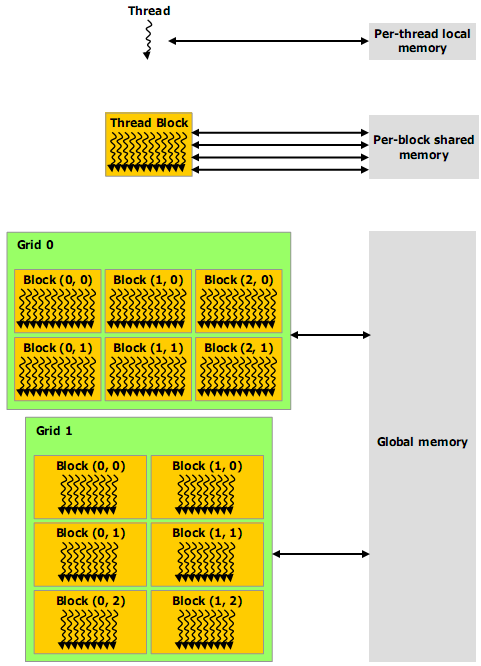
\includegraphics[width=.5\textwidth]{MemoriaHierarchy.png}
      \caption{\label{fig:MemoriaHierarchy}Jerarquía de hilos y patrones de acceso}
      %\caption{Jerarquía de hilos y patrones de acceso a los distintos tipos de memoria}
   \end{center}
\end{figure}

Adicionalmente existen dos espacios de memoria de sólo lectura accesible por todos los hilos: la memoria de texturas y la memoria de constante, optimizadas para usos específicos. Las memorias global, de textura y constante persisten mientras el kernel permanezca en acción.

Asi como se puede identificar los hilos dentro de un bloque, se pueden identificar los bloques dentro de un grid, mediante una variable blockIdx que también puede ser un índice unidimensional, bidimensional o tridimensional.

\subsection{Sincronizaciones por Barrera}

Como los distintos hilos colaboran entre ellos y pueden compartir datos, se requieren directivas de sincronización. En CUDA se puede especificar una sincronización del tipo barrera, en la que todos los hilos esperan a que los demás lleguen al mismo punto.

\subsection{Kernel}

CUDA extiende el lenguaje permitiendo definir funciones llamadas \emph{kernels}, que cuando son invocadas, son ejecutadas N veces en paralelo por N diferente hilos de CUDA. Estas abstracciones permiten un granulado fino en el paralelismo de los datos y los hilos, conduciendo al programador a dividir el problema en subproblemas que pueden ser tratados independientemente y en paralelo por bloques de hilos, y su vez dividir estos subproblemas en elementos individuales que pueden ser resueltos en paralelo y de manera cooperativa por todos los hilos de un mismo bloque.

%\vspace{5 mm}

Esta estructura preserva la expresividad del lenguaje permitiendo que los hilos cooperen en la resolución de cada subproblema, y al mismo tiempo permite la escalabilidad. En efecto, cada bloque de hilos puede ser programado en cualquier núcleo de procesamiento que este disponible, en cualquier orden, concurrente o secuencialmente. Por lo que cualquier programa CUDA ya compilado puede ejecutarse en sistemas con distinto número de núcleos de procesamiento, y solo el sistema de tiempo de ejecución debe conocer el dicho número de núcleos físicos. Todo esto desde el punto de vista del programador consiste en la extensión del lenguaje con un conjunto reducido de instrucciones, lo que supone un curva de aprendizaje suave; cabe notar, sin embargo, que a pesar de que CUDA permite la programación de kernels con pocas restricciones sobre el lenguaje, es necesario adoptar ciertas pautas a la hora de generar los kernels de las aplicaciones de interés, ya que de no seguir estas directrices el rendimiento se verá afectado severamente. Existen varias de ellas, pero las más importantes son dos: garantizar la coalescencia en el acceso a memoria (tanto en operaciones de lectura como de escritura) y usar la memoria compartida común a los hilos de un mismo bloque, para aprovechar su mayor velocidad de acceso en comparación con la memoria global del dispositivo \cite{cbestpractices}. Si se tienen en cuenta ambas características, es muy probable que el kernel en cuestión tenga un rendimiento excelente.

\section{Computación con PyCUDA}

\subsection{Requerimientos previos}

Antes de nada, es conveniente mencionar que para poder utilizar PyCUDA en una determinada máquina de pruebas, es necesario proveer primero de todo un framework asociado que necesita dicho software. En líneas generales, PyCUDA necesita obviamente de Python instalado en el sistema, así como de \emph{NumPy/SciPy} y de las librerías \emph{boost}. Estos a su vez tienen algunas dependencias de software con la que se debe tener cuidado, ya que de la correcta configuración de ATLAS y LAPACK, por ejemplo, va a depender en buena medida el rendimiento posterior de PyCUDA. Asimismo, para el ejemplo práctico del desarrollo de un algoritmo de detección de movimiento, se impone la necesidad de disponer de algunas librerías externas que faciliten sobremanera el manejo de imágenes y videos de manera suficientemente transparente para el usuario, como es el caso de PIL y OpenCV; y todo esto en su conjunto debe hacer uso de las librerias que proporciona la SDK de NVIDIA. En la figura \ref{fig:installedDependecies} se representan de manera clara estas dependencias de software.

\begin{figure}
   \begin{center}
      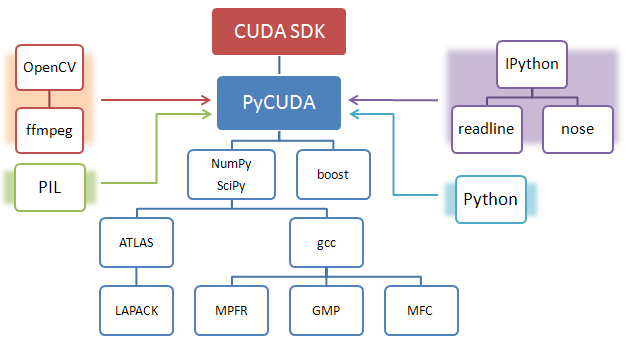
\includegraphics[width=.5\textwidth]{installedDependecies.png}
      \caption{\label{fig:installedDependecies} Software necesario para ejecutar PyCUDA}
      %\caption{\label{fig:installedDependecies} Jerarquía de software necesario para ejecutar PyCUDA}
   \end{center}
\end{figure}

\subsection{Ejecución de un kernel con PyCUDA}

No existe una única manera de ejecutar un algoritmo en un dispositivo con PyCUDA y, por supuesto, no todas resultan igual de eficientes. A continuación, se mostrará una sencilla secuencia de instrucciones que ilustran de manera bastante exacta el nivel de abstracción que puede llegar a alcanzarse sin menoscabo de la eficiencia.

%\vspace{5pt}

En primer lugar, se importan los mínimos paquetes necesarios para el funcionamiento de PyCUDA:

\begin{lstlisting}
import pycuda.autoinit
import pycuda.driver as cuda
from pycuda.compiler 
            import SourceModule
\end{lstlisting}

%\vspace{5pt}
Conviene hacer notar que aunque {\tt pycuda.autoinit} se encarga de inicializar el dispositivo (seleccionando el de mayor capacidad de cómputo si hay más de uno), así como de crear un contexto automáticamente, ambos aspectos pueden ser configurados manualmente.

%\vspace{5pt}

El siguiente paso consiste en cargar en memoria los datos que se desean procesar. En este punto, resulta muy aconsejable el uso del paquete {\tt NumPy} de la librería {\tt SciPy}, pues está provisto del potente tipo de dato {\tt numpy.array}, que facilita la preparación y manipulación de los datos. En este ejemplo, consideraremos dos arrays aleatorios \emph{a} y \emph{b}, cuyas componentes se restan dos a dos sobreescribiendo \emph{b} con el resultado.

%\vspace{5pt}

\begin{lstlisting}
import numpy as np
a = np.random.randn(16)
b = np.random.randn(16)
\end{lstlisting}

Aunque las más recientes GPUs soportan números en coma flotante de doble precisión, la mayoría de los dispositivos disponibles actualmente sólo soportan precisión simple, por lo que se impone la siguiente conversión de tipos:

\begin{lstlisting}
a.astype(np.float32)
b.astype(np.float32)
\end{lstlisting}

Una vez cargados los datos en memoria, los siguientes pasos son transferirlos al dispositivo y ejecutar el kernel. Con PyCUDA, ambos pasos pueden concentrar en uno solo, porque en la propia llamada al kernel puede estar implícita la transferencia de los datos a la memoria del dispositivo si se hace uso de la clase {\tt ArgumentHandler} disponible en {\tt pycuda.driver}, la cual está preparada para trabajar con arrays numpy como argumentos de entrada/salida.

\begin{lstlisting}
kernel = SourceModule("""
  __global__ void name(float *a, 
                       float *b) {
    int idx = threadIdx.x;
    b[idx] = b[idx] + a[idx];
  }
  """)
f = kernel.get_function("name")
f(cuda.In(a), cuda.InOut(b), 
  block=(16,16,1))
\end{lstlisting}

\subsection{\emph{Overhead} inducido}

Obviamente, el hecho de trabajar con un lenguaje interpretado como lo es Python, y con un \emph{wrapper} como lo es PyCUDA, implica una carga de trabajo extra para el procesador (no directamente relacionado con el cómputo en GPU) que debe ser analizada y comparada con la misma ejecución nominal en C para determinar si este \emph{overhead} supone un gravamen aceptable o no. En la figura \ref{fig:overhead-convolucion} se puede observar una comparación al ejecutar un filtro de convolución separable \cite{imagecuda} tanto en C como en Python + PyCUDA, separando en cada caso (para distintos tamaños de matrices cuadradas) el tiempo empleado en ejecutar únicamente el kernel en GPU y el programa completo (que engloba reserva de memoria, creacion de los arrays aleatorios, instanciacion del kernel, liberacion de memoria... así como el tiempo de ejecución del propio kernel en la GPU). Como se puede observar, y como era de esperar, los kernels se ejecutan siempre ligeramente más rápidos en C (un 50\% más rápido como mínimo, aunque hay que recordar que en estos niveles se habla de milisegundos para procesar matrices cuadradas del orden de 2048x2048 elementos). Sin embargo, en el tiempo total de ejecución se puede observar como lo que a priori debería ser una ventaja para C, a partir de 2048x2048 elementos el programa en C tarda de hecho más que el mismo programa en Python. Esto puede deberse a diversas razones: en C, los arrays a procesar se rellenan con números aleatorios obtenidos mediante la función {\tt rand()}, mientras que en Python es NumPy el encargado de generar las matrices aleatorias. Es conocida la gran eficiencia de NumPy a la hora de manejar matrices de gran tamaño, por lo que este detalle puede jugar a su favor. Otro posible punto de divergencia (ya que aunque los programas sean funcionalmente iguales, evidentemente hay ciertos elementos del lenguaje que están programados de forma distinta) sea la utilización de los timers propios de NVIDIA para realizar las medidas en C (a través de la librería proporcionada por la SDK {\tt shrUtils}); sería interesante comprobar hasta que punto están o no interfiriendo estos timers particulares en las mediciones totales.

%\vspace{5 mm}

En cualquier caso, puede comprobarse como el overhead que introduce la utilización de Python + PyCUDA no es, en ningún caso, alarmante. Sí que es necesario hacer notar, sin embargo, que en el caso de las primeras ejecuciones de algún programa que use PyCUDA, la fase de carga de los {\tt import} iniciales sí que es importante, llegando a tardar los mismos ejemplos de la figura \ref{fig:overhead-convolucion} cerca de 2 segundos, y donde la mayoría de los cuales se emplea en la precarga de estas directivas del \emph{wrapper}: comunicación inicial con el/los dispositivos existentes, selección de dispositivo, carga de la interfaz con el compilador de NVIDIA {\tt nvcc}, etc.

\begin{figure}
   \begin{center}
      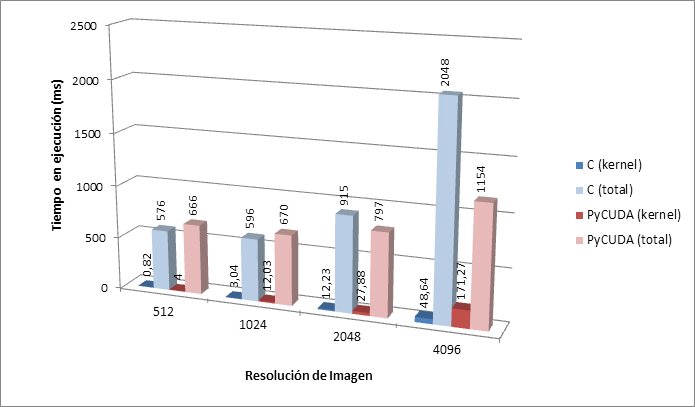
\includegraphics[width=.5\textwidth]{overhead-convolucion.png}
      \caption{\label{fig:overhead-convolucion}Kernel para un filtro de convolución: C y PyCUDA}
      %\caption{\label{fig:overhead-convolucion}Comparación de tiempos al ejecutar un kernel de convolución sobre C y sobre PyCUDA}
   \end{center}
\end{figure}


\section{Producto matricial}

La manera tradicional de abordar la multiplicación de matrices pasa por ejecutar un algoritmo secuencial de complejidad casi cúbica en las mejores implementaciones. Su versión paralela, en cambio, permite el cálculo simultáneo de las filas de la primera matriz multiplicando con la correspondiente columna de la segunda para formar el resultado.

%\vspace{5 mm}

BLAS (Basic Linear Algebra Subprograms) es, de facto, una interfaz estándar de programación de librerías que realizan operaciones básicas de álgebra lineal con vectores y/o matrices.

%\vspace{5 mm}

Desde su primera publicación, en 1979, numerosos fabricantes de hardware han desarrollado versiones altamente optimizadas de BLAS. También NVIDIA lo ha incluido en el SDK de CUDA para proporcionar una versión de altas prestaciones para estas operaciones. Dicha implementación ha sido denominada CUBLAS.

%\vspace{5 mm}

Por su parte, PyCUBLAS es un wrapper \cite{pycublas} de Python para CUBLAS creado por Derek Anderson que ha centrado su diseño en la multiplicación de grandes matrices. Dispone, además, de las ventajas ya comentadas de Python en cuanto a abstracción, lo que posibilita la ejecución de una operación con muy pocas líneas de código.

\begin{lstlisting}
import numpy as np
from pycublas import CUBLASMatrix

a = np.random.randn(width,length).
              astype(np.float32)
b = np.random.randn(width,length).
              astype(np.float32)

a = CUBLASMatrix(np.mat(a))
b = CUBLASMatrix(np.mat(b))

c = a * b
\end{lstlisting}

Esta sencillez sintáctica podría ser atractiva para extender el uso de CUDA entre investigadores de otras ciencias cuyos estudios precisen de la manipulación de cantidades masivas de datos. 

\begin{figure}[t]
   \begin{center}
      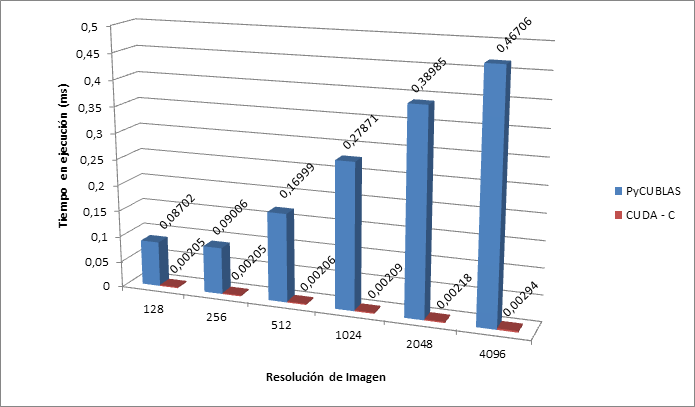
\includegraphics[width=.5\textwidth]{pycublas.png}
      \caption{\label{fig:pycublas}Producto de matrices en CUDA: C y PyCUBLAS}
      %\caption{\label{fig:pycublas}Comparación de tiepos de ejecución al computar el producto de matrices cuadradras entre implementación nativa de CUDA en C y PyCUBLAS}
   \end{center}
\end{figure}

%\vspace{5 mm}

En esta sección se confrontan el tiempo de ejecución en el dispositivo de una multiplicación de matrices cuadradas de diferentes dimensiones, tanto a través de PyCUBLAS como de su correspondiente versión nativa en C. No se ha contemplado en la gráfica de la figura \ref{fig:pycublas} los tiempos de ejecución en la CPU, puesto que estos llegan a ser hasta 35 millones de veces mayor en el caso de una matrix de 2048x2048.


\begin{figure*}[t]
   \begin{center}
      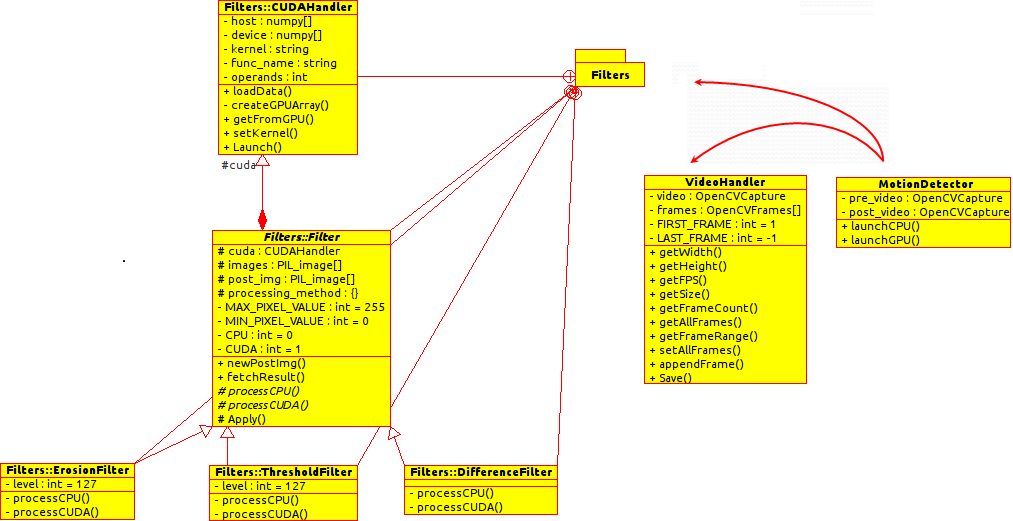
\includegraphics[width=.9\textwidth]{UML.png}
      \caption{\label{fig:UML}Jerarquía de clases del detector de movimiento}
   \end{center}
\end{figure*}
\section{Detección de movimiento}

Teniendo en cuenta las posibilidades del modelo CUDA exploradas hasta ahora, parece lógico buscar algún algoritmo que conlleve un esfuerzo computacional notable para ir un paso más allá en la exploración del uso de Python como vehículo conductor de los programas de cómputo. Una primera consideración interesante es el RANSAC \cite{Jiayin:2010:CMD:1933304.1933936}, un algoritmo utilizado frecuentemente en campos muy diversos, pero no resulta fácilmente acomodable al cómputo paralelo bajo esta arquitectura debido a que requiere de estructuras de datos complejas que además contemplan múltiples dependencias entre ellas.

%\vspace{5 mm}


Finalmente, se ha escogido como objetivo de desarrollo el diseño e implementación de un paquete que permita aplicar diferentes filtros a una imagen, a un conjunto de imágenes o a un video, en cuyo caso será descompuesto en sus correspondientes frames. Este paquete puede utilizarse para acelerar el cálculo de aplicaciones complejas que requieran de la aplicación de filtros \cite{DBLP:conf/csse/YangZP08}. En concreto, una de las más interesantes consiste en un programa de detección de movimiento: a grandes rasgos, toma 2 frames de un video y discierne (marcando en color rojo sobre uno de los frames original) las partes en movimiento entre los mismos. Esto mismo se ejecuta de manera iterativa el número de veces necesario para realizar la detección de movimiento sobre un video compuesto de una multitud de frames.

%\vspace{5 mm}

El paquete Filters desarrollado para este fin se estructura, esencialmente, en torno a dos clases: CUDAHandler, concebido para abstraer de muchos detalles de la comunicación con la GPU (informalmente, podría considerarse un \emph{wrapper} del propio  PyCUDA); y Filter, clase abstracta de la que heredan cada uno de los filtros implementados. En la figura \ref{fig:UML}, pueden observarse tres clases hijas de Filter que contienen las instrucciones para gestionar tres filtros necesarios para la detección de movimiento (\emph{Difference}, \emph{Threshold} y \emph{Erosion}), como se explica en la posterior subsección. También se contempla una clase MotionDetector, encargada de dirigir la detección en sí aplicando los filtros frame tras frame y que hace uso del paquete Filters, además por último de la clase VideoHandler que la abstrae de la manipulación de las operaciones de gestión de vídeo.


\subsection{Implementación del algoritmo}

El algoritmo de detección de movimiento más simple se basa en la aplicación de una secuencia de filtros sobre los frames (imágenes) del video \cite{codeproject}.
Para entender el proceso basta con escoger 2 frames consecutivos del video y aplicar los siguientes pasos:

\begin{enumerate}
   \item Conversión a escala de grises de las 2 imágenes
   \item Aplicación del filtro de diferencia a las 2 imágenes
   \item Aplicación del filtro Threshold
   \item Aplicación del filtro de Erosión
   \item Mezcla en el canal R de la imagen original con la imagen resultado de los filtros
\end{enumerate}


Una vez obtenidos las 2 imágenes en escala de grises, se procede a aplicar el primer filtro:

\textbf{Filtro de Diferencia:} Este filtro consiste en el valor absoluto de la resta de cada píxel (restando canal a canal en caso de imágenes de varios canales) de las dos imágenes. Con esto obtenemos las zonas donde se ha producido movimiento, como se puede observar en la primera imagen de la figura \ref{fig:joined}.

%\vspace{5 mm}

\textbf{Filtro Threshold:} La finalidad de este filtro es obtener una imagen binaria donde solo aparecen píxeles blancos o negros. Este filtro compara cada píxel con un umbral, y si el valor del píxel está por debajo se asigna el valor 0 (negro), en caso contrario (por encima del umbral) se asigna el valor 255 (blanco). Así pues, la imagen resultante quedaría como la segunda imagen de la figura \ref{fig:joined}, donde además se aprecia la aparición de ruido a simple vista.

%\vspace{5 mm}

\textbf{Filtro de Erosión:} Contenido dentro los llamados Filtros Morfológicos, este filtro determina si un píxel se mantiene (se define como blanco) o se elimina (se define como negro). Para sopesar esta decisión se hace uso de una máscara (definida a conveniencia) que determina los píxeles vecinos a examinar; desde que al menos uno de estos vecinos esté en negro, se elimina el píxel analizado (operación \emph{and} lógica. Por el contrario, si todos los píxeles vecinos existen el píxel analizado permanecerá en blanco. El objetivo de aplicar este filtro es eliminar el ruido expuesto por el filtro anterior, como se puede apreciar en la tercera imagen de la figura \ref{fig:joined}.

%\vspace{5 mm}

Por último, queda realizar el fundido en el canal R de la imagen original con la imagen resultante de aplicar el filtro de erosión. Este fundido no es más que una suma de píxel a píxel, obteniendo así el resultado final de la figura \ref{fig:joined}.

\begin{figure}[t]
   \begin{center}
      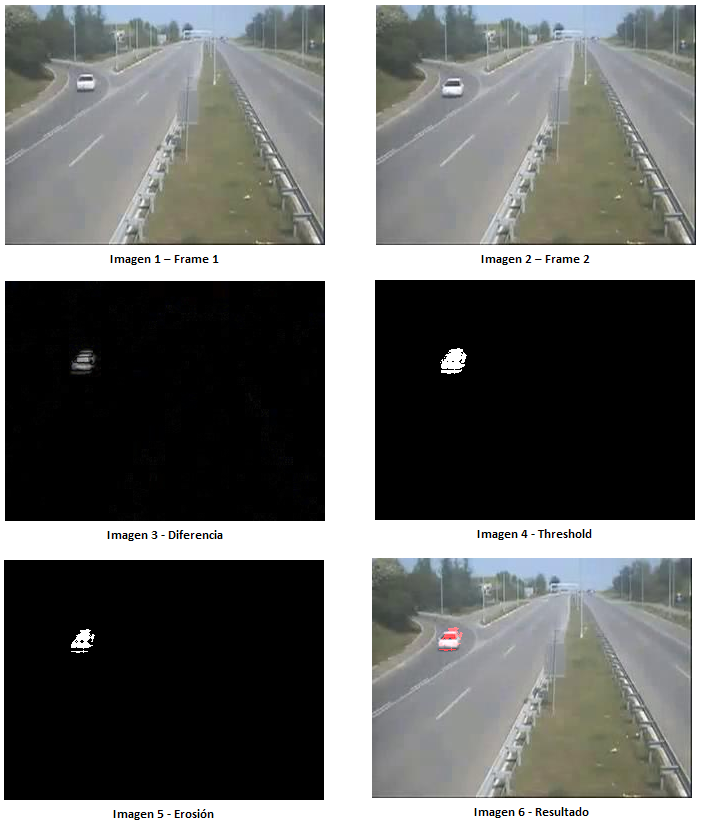
\includegraphics[width=.5\textwidth]{joined.png}
      \caption{\label{fig:joined}Fases del algoritmo de detección de movimiento}
   \end{center}
\end{figure}

\balance
\section{Conclusiones}

Como se ha podido observar, implementar la resoluci\'{o}n de problemas relativamente complejos no es especialmente costoso en tiempo con lenguajes din\'{a}micos como Python. Si a eso se le a\~{n}ade la posibilidad de utilizar todo el potencial de c\'{o}mputo paralelo que ofrece CUDA a trav\'{e}s de \emph{wrappers} como PyCUDA, el resultado es una herramienta muy potente que puede satisfacer las necesidades de investigadores y cient\'{i}ficos en general tanto por madurez de la misma como por rendimiento, a cambio de un peque\~{n}o e inevitable \emph{overhead} inherente a la naturaleza interpretada de Python y al uso de \emph{wrappers}. De cualquier forma, dicho incremento en tiempo es lo suficientemente despreciable para que se pueda ignorar sin temor, m\'{a}xime si se tiene en cuenta el hecho de que a mayor tama\~{n}o del problema, m\'{a}s imperceptible se torna dicha carga de trabajo adicional. Por \'{u}ltimo, pero no por ello menos importante, los autores desean recalcar que la curva de aprendizaje necesaria para poder manejarse en este entorno con cierta solvencia es considerablemente m\'{a}s suave que la que conlleva el entorno tradicional de programaci\'{o}n de CUDA bajo C/C++, lo cual consideran un argumento de suma importancia para atraer usuarios potenciales, sean acad\'{e}micos de nueva hornada o investigadores asentados que tienen necesidad de c\'{a}lculo masivo paralelo y que utilizan para ello aplicaciones desarrolladas hace a\~{n}os en lenguajes como FORTRAN cuyo mantenimiento se hace cada vez m\'{a}s inviable. En definitiva, si se tiene intenci\'{o}n de migrar estas aplicaciones, Python y PyCUDA conforman una alternativa perfectamente capaz.

\bibliographystyle{Jornadas}
\bibliography{pycuda}

\end{document}

